\documentclass[12pt]{article}
\usepackage{fancyhdr}
\usepackage{datetime}
\usepackage{enumitem}
\usepackage{float}
\usepackage{graphicx}
\graphicspath{ {images/} }
%\usepackage{showframe}

%custom variables
\newdate{date}{11}{10}{2016}
\newcommand{\hwNum}{No.3}
\newcommand{\assignmenttype}{Lab}

%adjusting vertical whitespace for the images at the top
\makeatletter
\setlength{\@fptop}{0pt}
\makeatother


%header
\pagestyle{fancy}
\lhead{Daniel Andronov}
\chead{\thepage}
\rhead{\assignmenttype \hwNum}
\cfoot{\thepage}

\fancyheadoffset[LO,RE]{1pt}
\fancyheadoffset[RO,LE]{1pt}

%titlepage
\title{\assignmenttype}
\author{Daniel Andronov}
\date{\displaydate{date}}

%addition settings
\topmargin=-0.45in
\evensidemargin=0in
\oddsidemargin=0in
\textwidth=6.5in
\textheight=9.0in
\headsep=0.25in

%start the sections from 3
\setcounter{section}{3}
\setcounter{subsection}{-1}

%enumerate left margin
\setlist[enumerate,1]{leftmargin=2.9cm}

\begin{document}
\maketitle
\newpage

\subsection{Prelab}
\begin{enumerate}[label=\textbf{Question \arabic*)}]
	\item  \begin{enumerate}[label=\alph*)]
			\item False, each object needs its own request.  
			\item True, if using HTTP 1.1, the connection will not be closed until the client says so. 
			\item False, after each response, the connection is closed. 
			\item False, that field indicates when the packet was sent.
		\end{enumerate}
	\item  \begin{enumerate}[label=\alph*)]
			\item The end-to-end delay would be $2N + 2$ RTT, where RTT is the round trip time. Two RTT's for setting up the connection and getting the base
			\item If using HTTP 1.1, the end-to-end delay woudl be $N+2$ RTT, 2 RTT for setting up the connection and the base HTML file, and N RTT for each subsequent object.
			\item If usine HTTP 1.0 \& four parallel connections, then the end-to-end delay would be $2N/4$ or $N/2$. 
		\end{enumerate}
	\item The most modern iteration of FTP is RFC 959. It's well known port numbers are 20 \& 21. FTP has two port numbers assigned to it because it was found the the useing the header to communicate commands and manage directories created too much latency. One connection is used to send commands and the other to move data.
	\item From the figure below, the \texttt{dig} command returned nine answers but ranked \texttt{relay.bu.edu} above the others. A secondary \texttt{dig} revealed that \texttt{dig} has several IP addresses, most like a redundacy safety measure, but the first was \texttt{128.197.228.27}. 
		\begin{figure}[h]
			\caption{The results of the \texttt{dig} queries.}
			\centering
			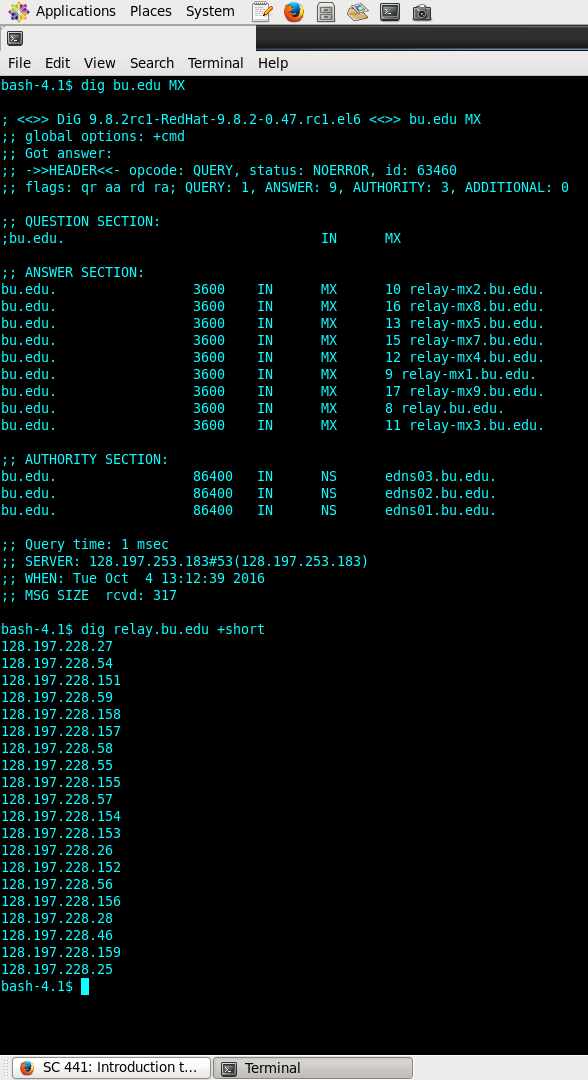
\includegraphics[scale=0.5]{dig}
		\end{figure}
\end{enumerate}

\subsection{HTTP}


\begin{enumerate}[label=\textbf{Question \arabic*) }]
	%Q1
	\item The browser is running HTTP1.1.\\ My computer's IP address is 172.16.160.130\\
	%Q2
	\item bc.edu's  IP address is 136.167.2.220\\
	%Q3
	\item The source port is 54910 and the destination port is 80.\\
	%Q4
	\item The source is now 80 and the destination is 54910. \\
	%Q5
	\item The server is running Apache.\\	The HTML file the was requested was last modified on Tuesday, October 4th 	2016 at 17:17:01 GMT.\\
	%Q6
	\item There were a total of 9 GET messages sent. This could be either for reduancy, so that if packets are lost, at least one will make it through the network to bc.edu in order to
 initiate a respone, or part of some parallelization of certain process that each send their own HTTP GET message.
\end{enumerate}


\subsection{DNS}
\begin{enumerate}[label=\textbf{Question \arabic*)}, resume]
	%Q7
	\item The query and response are both send via UDP.
	%Q8
	\item The source port is 42422 and the destination port is 53.
	%Q9
	\item The DNS query is sent to 172.16.160.2 and \texttt{dig} reveals that the DNS local server IP is the same
		\begin{figure}[h]
			\caption{The result of the dig command reports the local DNS IP }
			\centering
			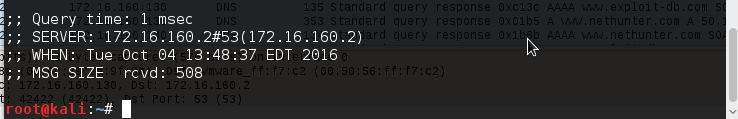
\includegraphics[scale = 0.75]{DNS_IP}
		\end{figure}
	%Q10
	\item The DNS query message is of type A, and contains no answers or records
	%Q11
	\item The DNS response message returns with 1 answer, 5 authority, and 8 additional records, for a total of 13 records. The first answer is the name and IP address of the desired name server as it is known in the cache. The authoratative records contain the names and IP address of authoratative name servers for the desired domain that contain the most current information. The additional records contain the TTL's of the authoratative records, as well as their names and IP addressess, as stored in the cache. 
	%Q12
	\item The maxiumum TTL of a DNS record in 86400 seconds or 3 years as the TTL number is a 32 bit value.
	%Q13
	\item Type "AAAA" queries request the IPv6 128 bit address instead of the regular 32 bit IPv4 address. It is defined by RFC 3596.
\end{enumerate}


\subsection{Authentication Mechanisms and HTTP}
\begin{enumerate}[label=\textbf{Question \arabic*)}, resume]
	%Q14
	\item The HTTP method POST was used to send the login information.
	%Q15
	\item The password was submitted in plain text, as per the below figure. This is a fairly serious security concern.
		\begin{figure}[h]
			\caption{This is the contents of the POST HTTP message that was used to send the login information}
			\center
			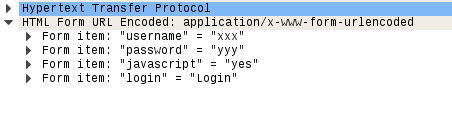
\includegraphics{http_login}
		\end{figure}
\end{enumerate}

\subsection{Cookies}
\begin{enumerate}[label=\textbf{Question \arabic*)}, resume]
	%Q16
	\item In the first HTTP GET message, there is no cookie ID as it was deleted when the history of the browser was cleared.
	%Q17
	\item The first HTTP response message sets the cookie ID to\\
	         \texttt{d07b4f1238bada427fb22ed41ccf23f9f1475768042}.
	%Q18
	\item In the second HTTP GET message, the cookie ID from the previous response is that which is included in the message. 
		\begin{figure}[!t]
			\caption{The cookie ID provided in the response message the initial GET message}
			\center
			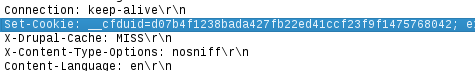
\includegraphics{http_cookie_resp}
			\caption{This figure shows that the cookie id in the subsequent HTTP GET message matches that which was given in the previous response}
			\center
			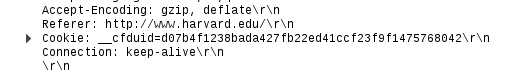
\includegraphics{http_cookie_get}
		\end{figure}
\end{enumerate}
\end{document}